
\documentclass[8pt]{article}

\usepackage[utf8]{inputenc}

\usepackage{amsmath, bm}
\usepackage{graphicx}
\usepackage{amssymb}
\usepackage{float}
\usepackage{caption}
\usepackage{subcaption}
% set font size to 11pt

% set margin
\usepackage[margin=0.5in]{geometry}

\setlength{\parskip}{\baselineskip}%
\setlength{\parindent}{0pt}%
\setlength{\voffset}{-0.75in}
\setlength{\headsep}{5pt}

\begin{document}

% insert pdf cover page here

\title{Lab report: 3A3 Supersonic Nozzle}
\author{lwp26}
\date{October 2023}
\maketitle

\section{Part 1 Convergent - divergent nozzle}

\begin{figure}[H]
    \centering
    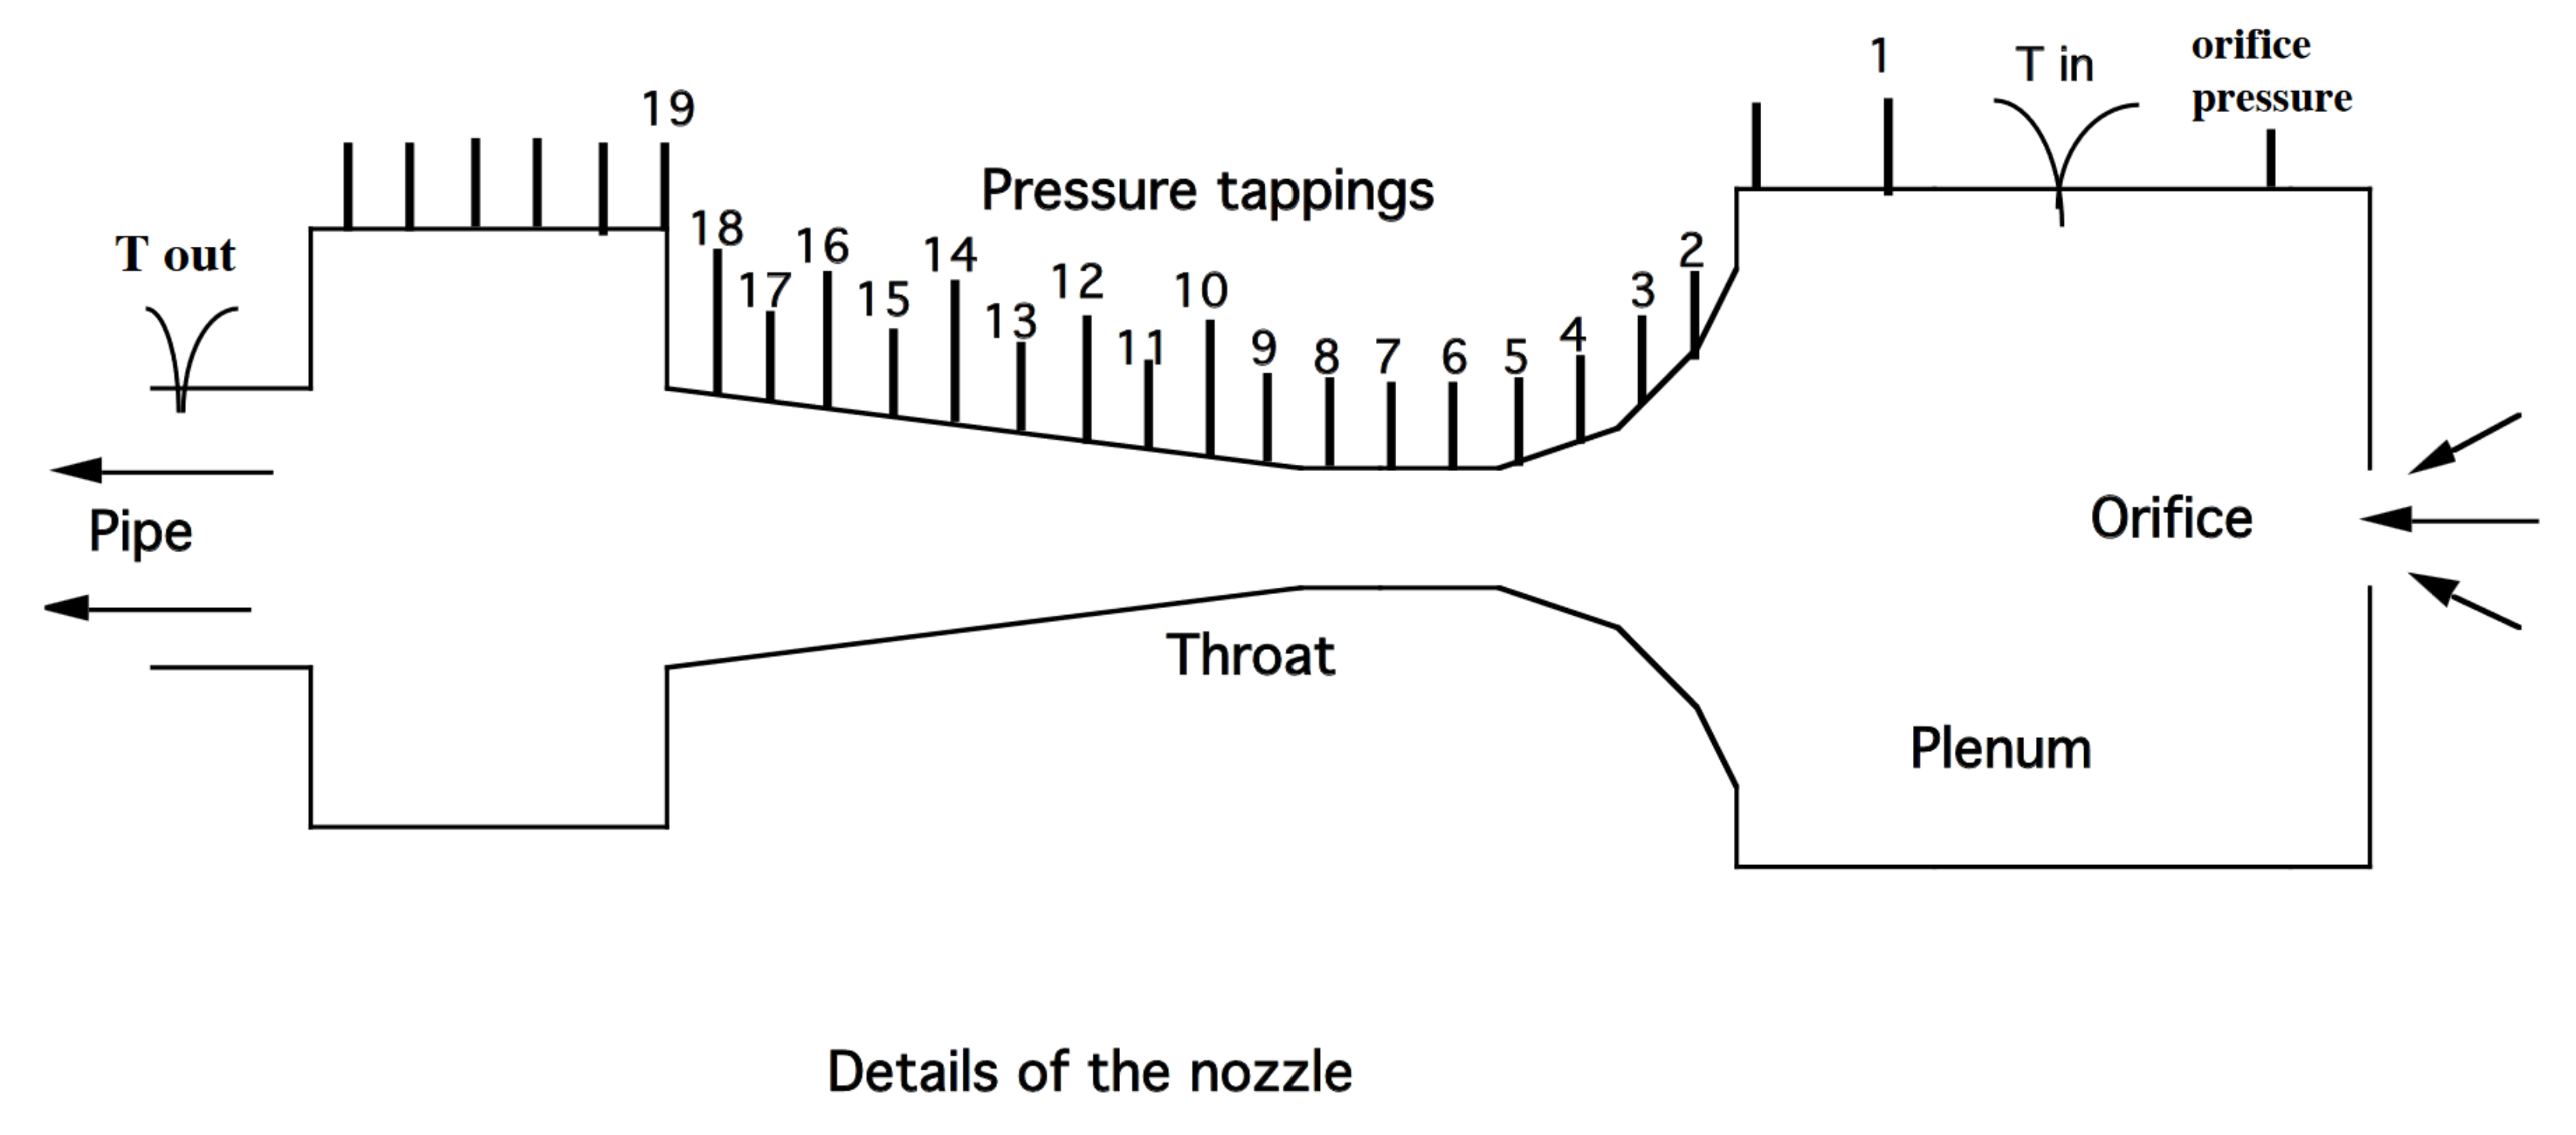
\includegraphics[width=0.8\textwidth]{small_nozzle_layout.png}
    \caption{Layout of Convergent - divergent nozzle}
    \label{fig:figure1}
\end{figure}

Orifice calibration: the diameter of the orifice is 17.47 mm. To a first approximation, assume that
\begin{itemize}
    \item The flow into the orifice is inviscid,
    \item the flow is slow enough to be treated as incompressible with density equal to that in the atmosphere upstream of the orifice (where the velocity is negligible),
    \item the velocity is uniform across the plane of the orifice,
\end{itemize} 

The first assumption is valid, due to the thin section of the orifice. This means that up to and including the small oriface surface, the flow can be treated as inviscid, and Bernoulli's equation can be applied.
The second assumption requires further justification (in my eyes). The flow upstream of the oriface has a negligible velocity compared to that of the oriface, and so the density of the flow upstream of the oriface is equal to that of the atmosphere.
However, the flow through the oriface may be compressible due to the high velocity of the flow.
If we assume the nozzil is choked upstream of the oriface, then its non-dimensional mass flow rate is given by the following equation.
\begin{equation}
    \frac{\dot{m}\sqrt{c_pT_0}}{p_0A^*} = 1.281
\end{equation}
From this, the non dimensional mass flow rate at the oriface can be calculated using the area ratio of the oriface to the nozzle throat.
The area of the throat was not known however, but can be assumed to be at least less than half the area of the oriface.
At this area ratio of $0.5$, the density ratio $\rho/\rho_0$ is greater than $0.9535$, and so the assumption that the flow is incompressible is crude but sufficient for the purposes of this experiment.

\newpage


The third assumption that the velocity is uniform across the plane of the oriface is valid, as the oriface is thin and the flow is inviscid.

With these assumptions, the theoretical flow rate through the orifice can be calculated using the pressure difference between the orifice plane and the upstream atmosphere is that measured on the
water manometer. From the Bernoulli equation,

\begin{equation}
    p_1 + \frac{1}{2} \rho v_1^2 = p_2 + 0
\end{equation}

where $A$ is the cross-sectional areas of the oriface. The theoretical flow rate through the orifice is then given by
\begin{equation}
    \dot{m} = \rho_a A v_2 = \rho_a \left( \frac{\pi D^2}{4}\right) \sqrt{\frac{2(p_2-p_1)}{\rho_a}} \;\;\;\;\;\; \text{where} \;\;\;\;\;\ p_2 - p_1 = \rho_w g \Delta h
\end{equation}
Where $\rho_a$ is the density of air and $\rho_w$ is the density of water used for the manometer.
However, the actual flow rate through the orifice differs from the theoretical value as our assumptions are not entirely valid.
This difference is characterised by the discharge coefficient $C_d$ which is defined as the ratio of the actual flow rate to the theoretical flow rate.
\begin{equation}
    \dot{m}_{actual} = C_d \dot{m}_{theoretical}
\end{equation}
% https://arc.aiaa.org/doi/pdf/10.2514/6.2019-3651 ?
The discharge coefficient of the oriface is effectively constant over the range of high reynolds numbers considered in this experiment. 

\begin{figure}[H]
    \centering
    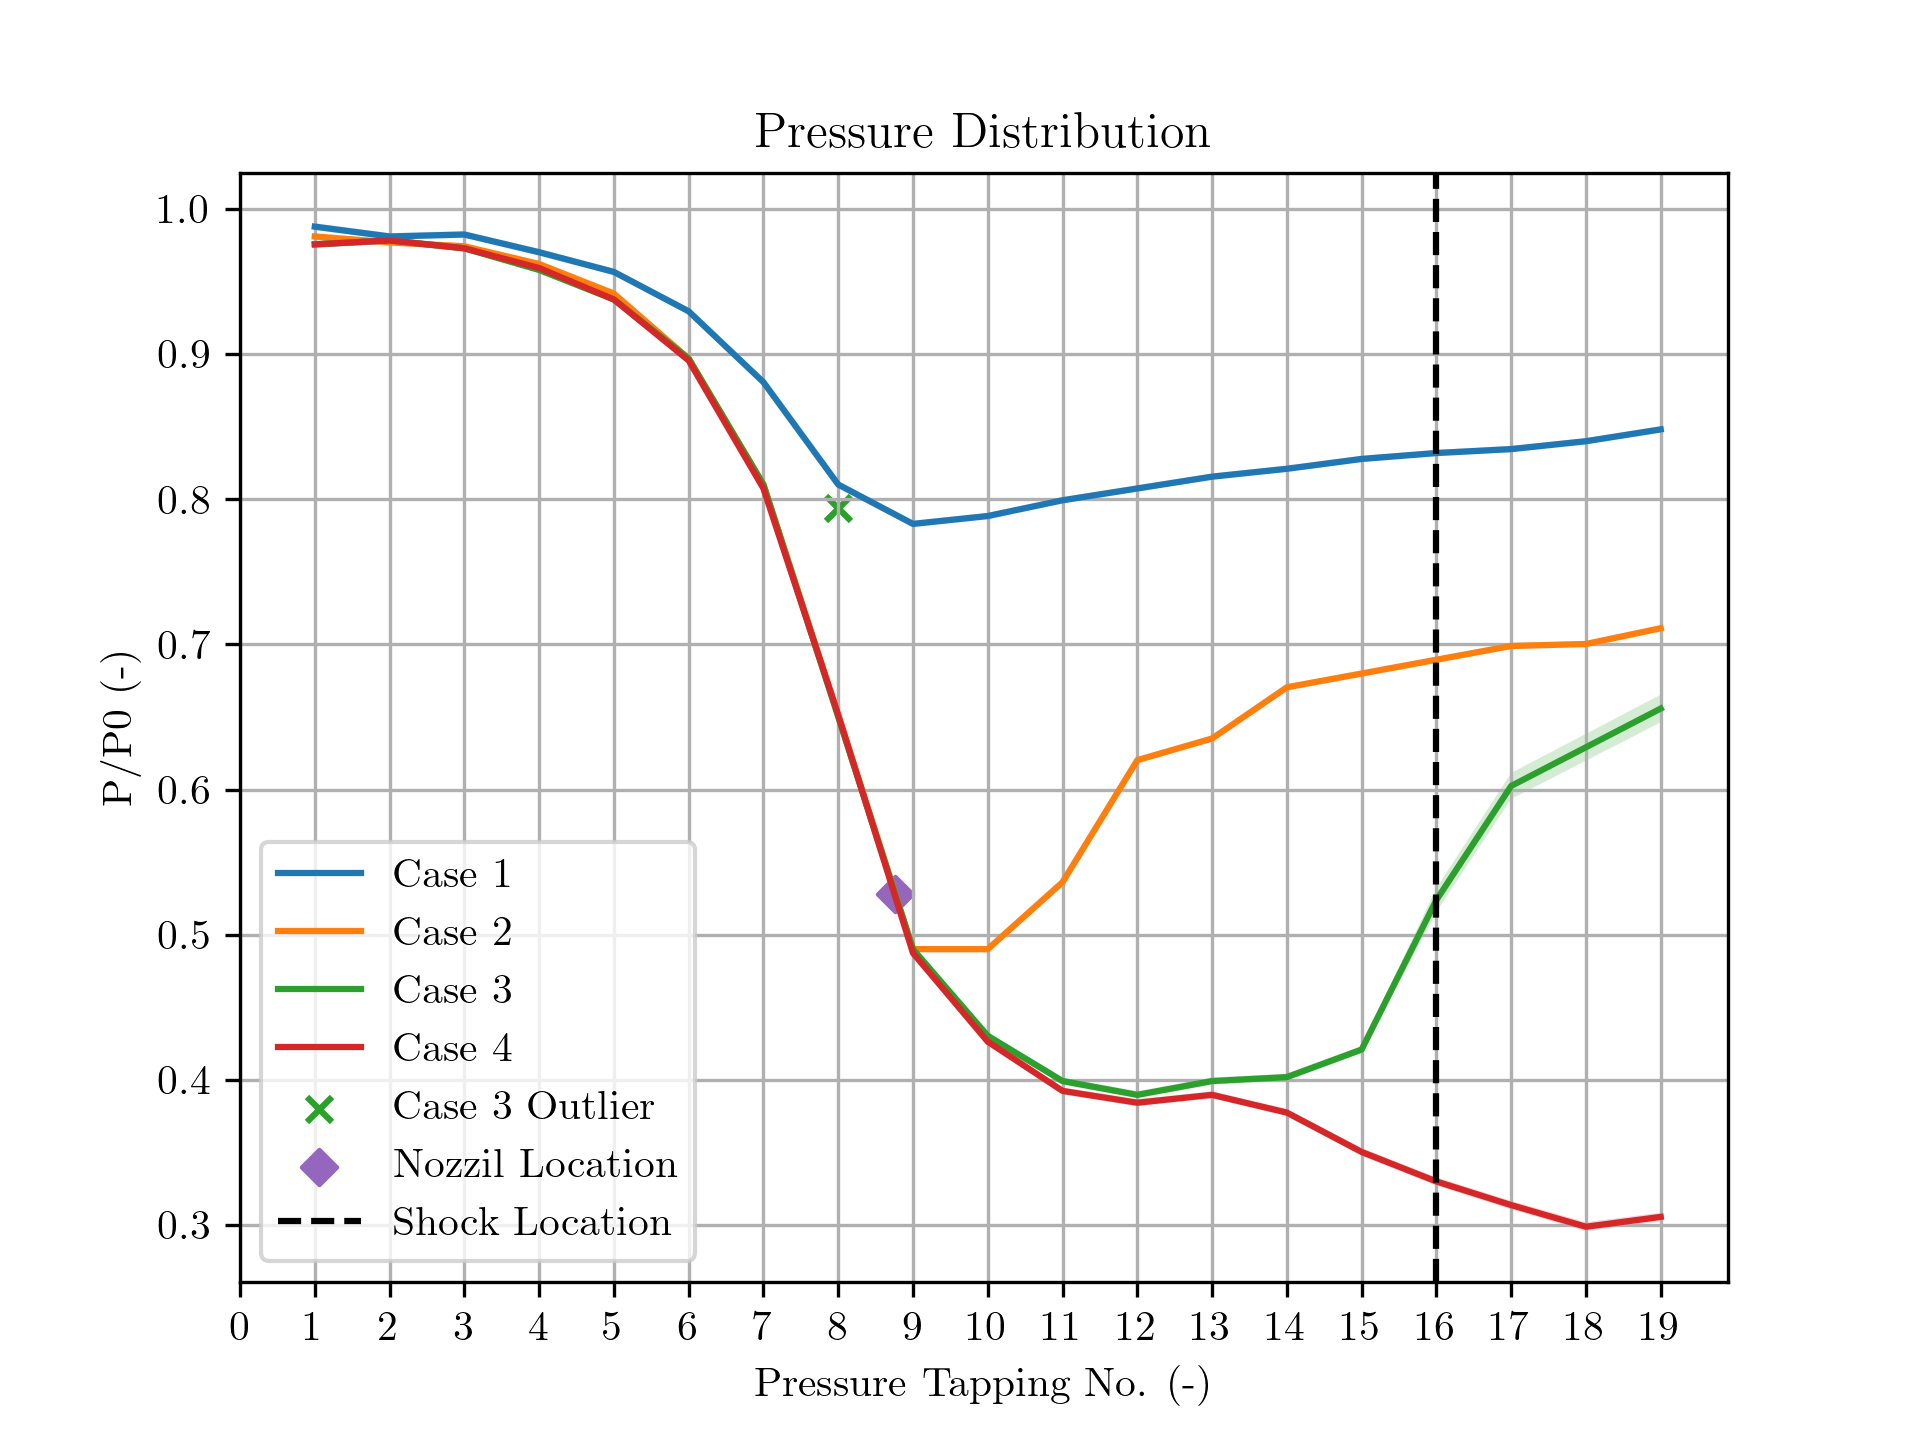
\includegraphics[width=0.8\textwidth]{pressure_ratio_distribution_corrected.png}
    \caption{Figure 1}
    \label{fig:figure4}
\end{figure}

\begin{figure}[H]
    \centering
    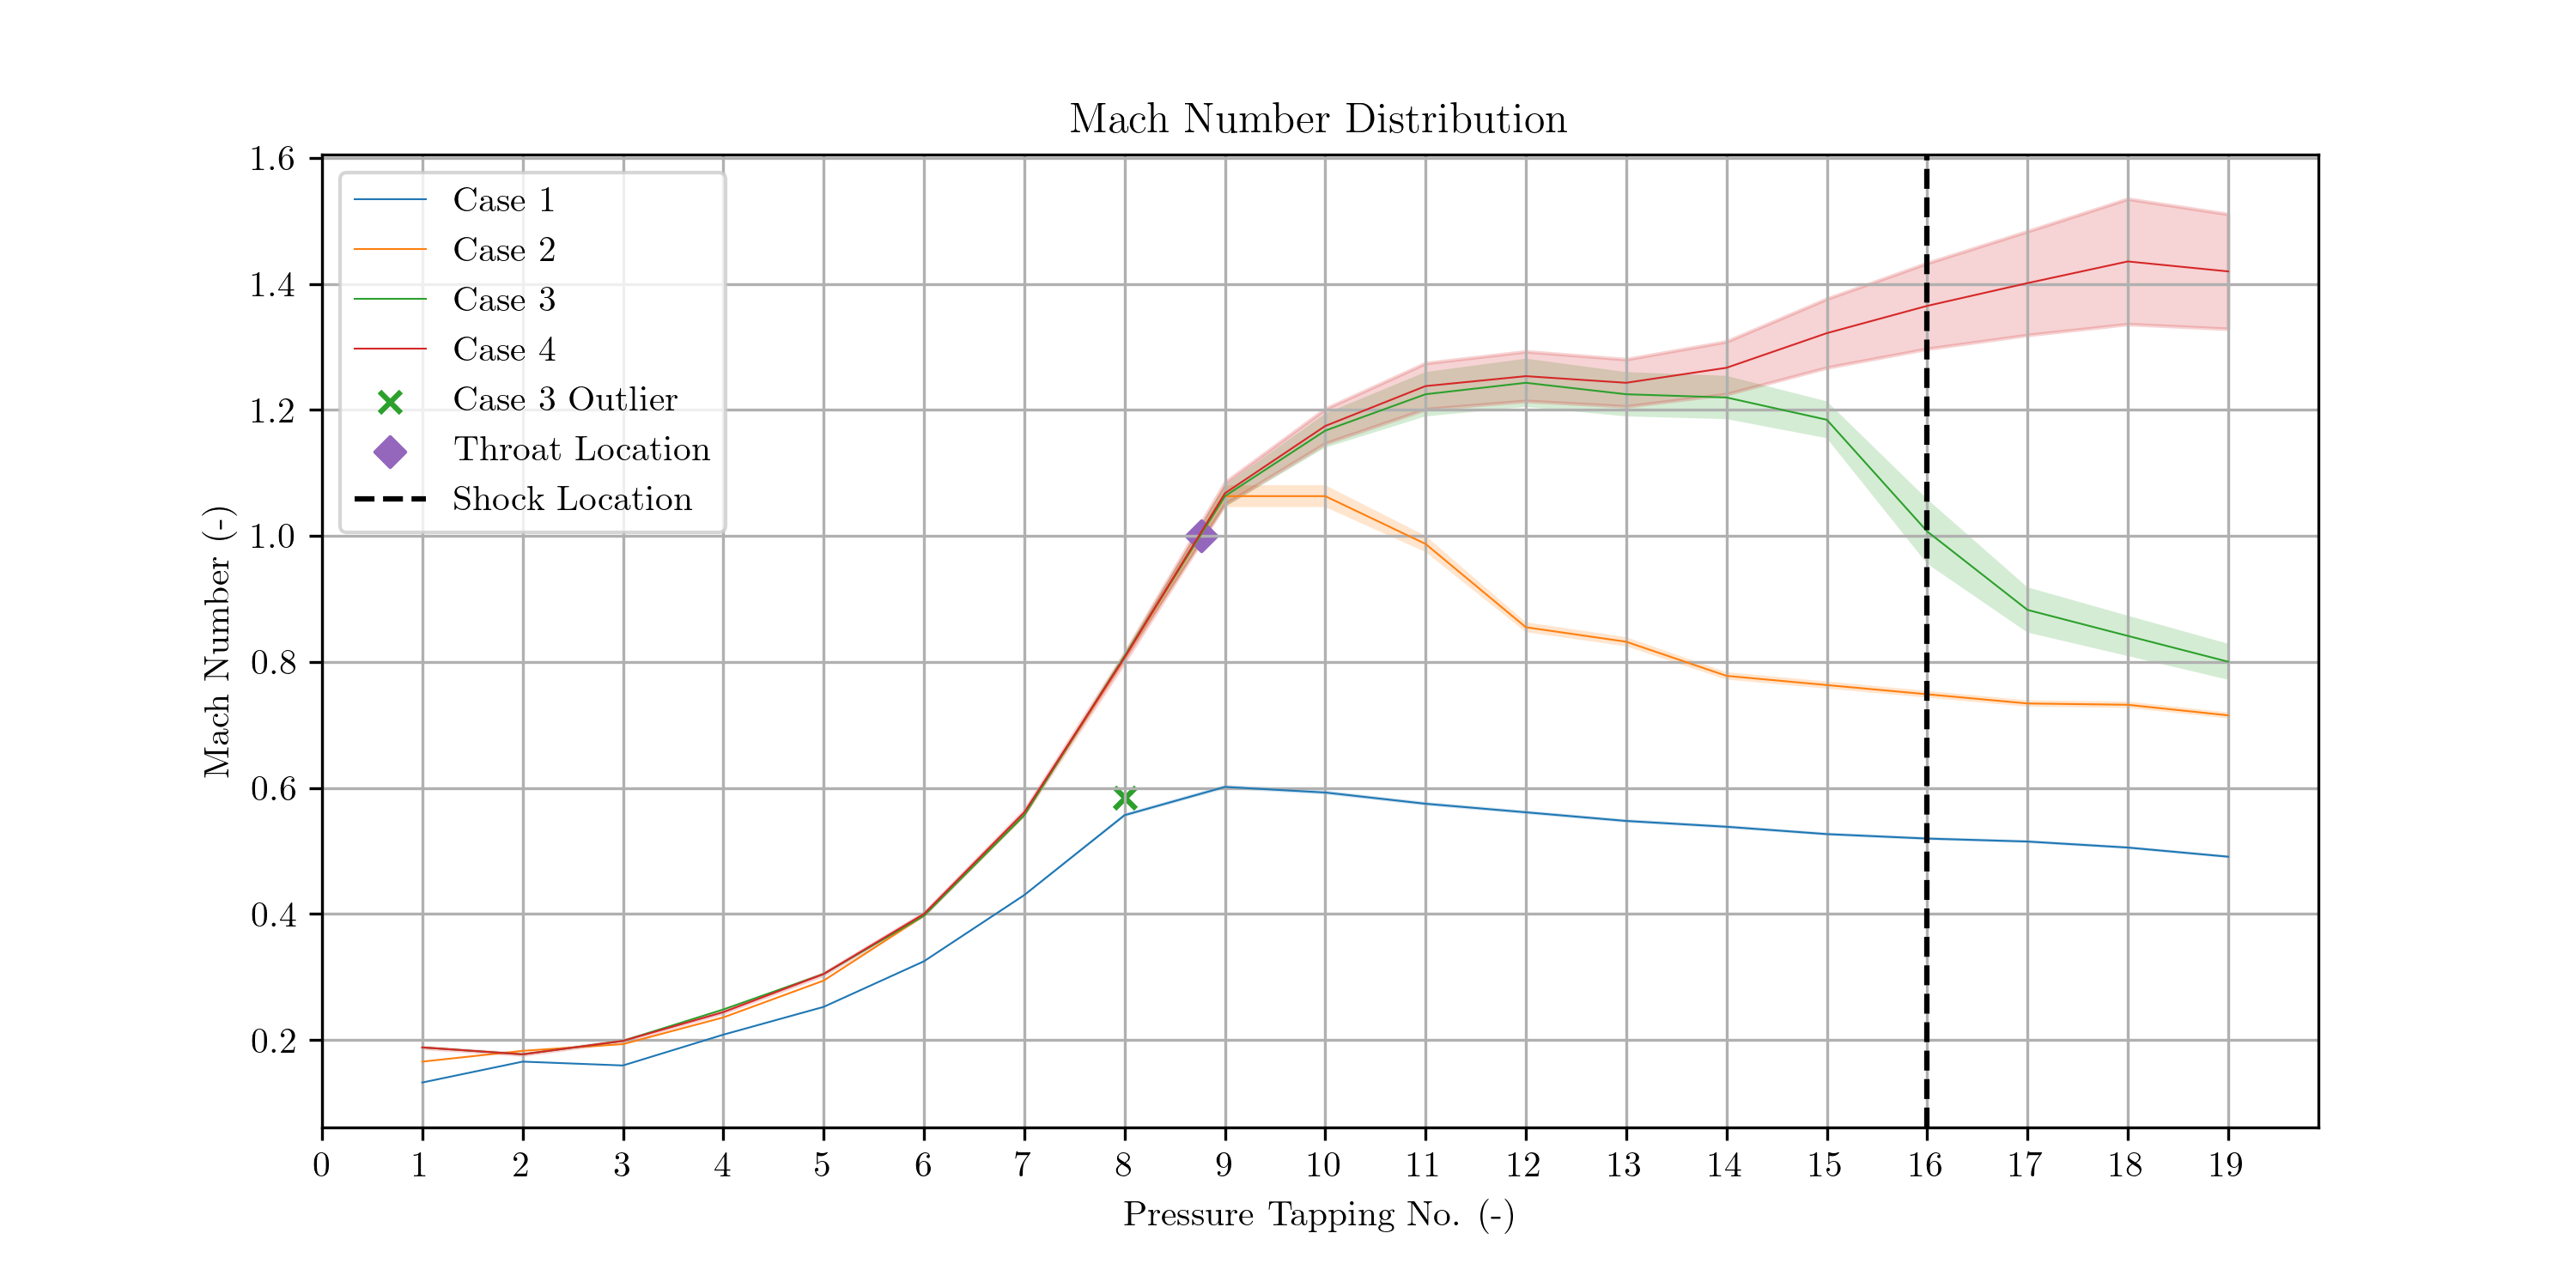
\includegraphics[width=0.8\textwidth]{mach_number_distribution_corrected.png}
    \caption{Figure 1}
    \label{fig:figure5}
\end{figure}

\begin{figure}[H]
    \centering
    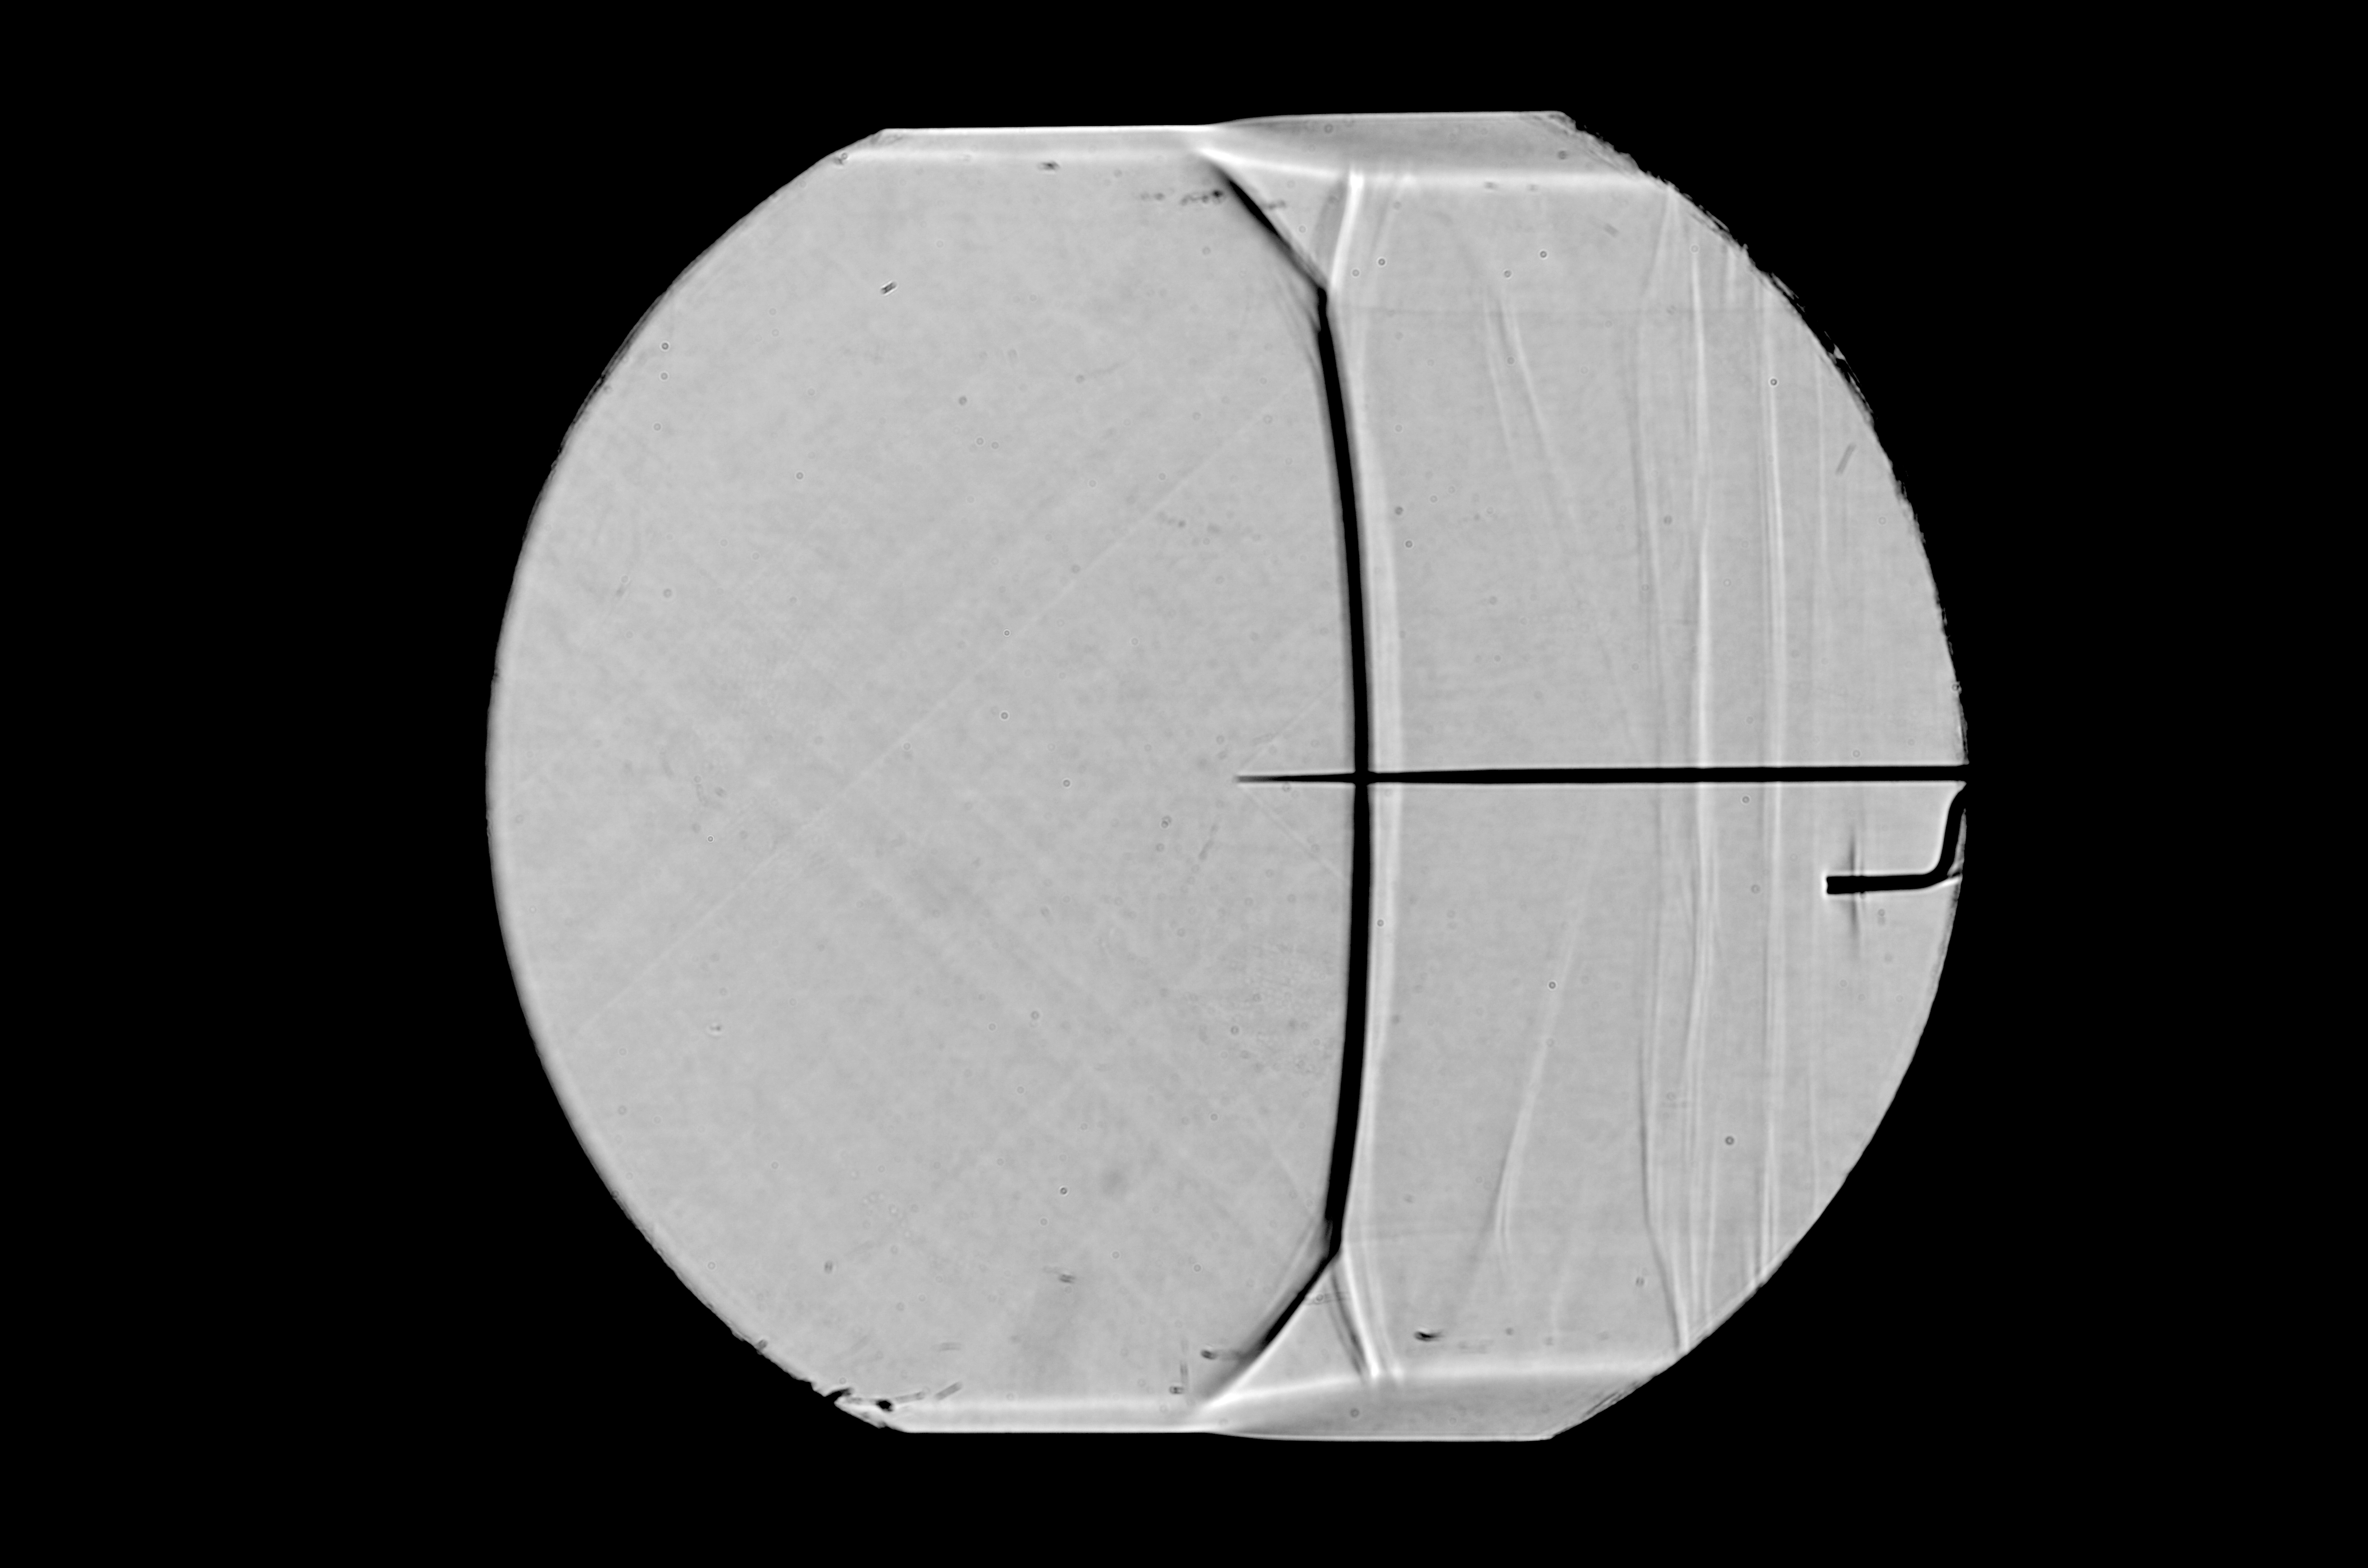
\includegraphics[width=0.8\textwidth]{starting_shock.jpg}
    \caption{Figure 1}
    \label{fig:figure6}
\end{figure}

\begin{figure}[H]
    \centering
    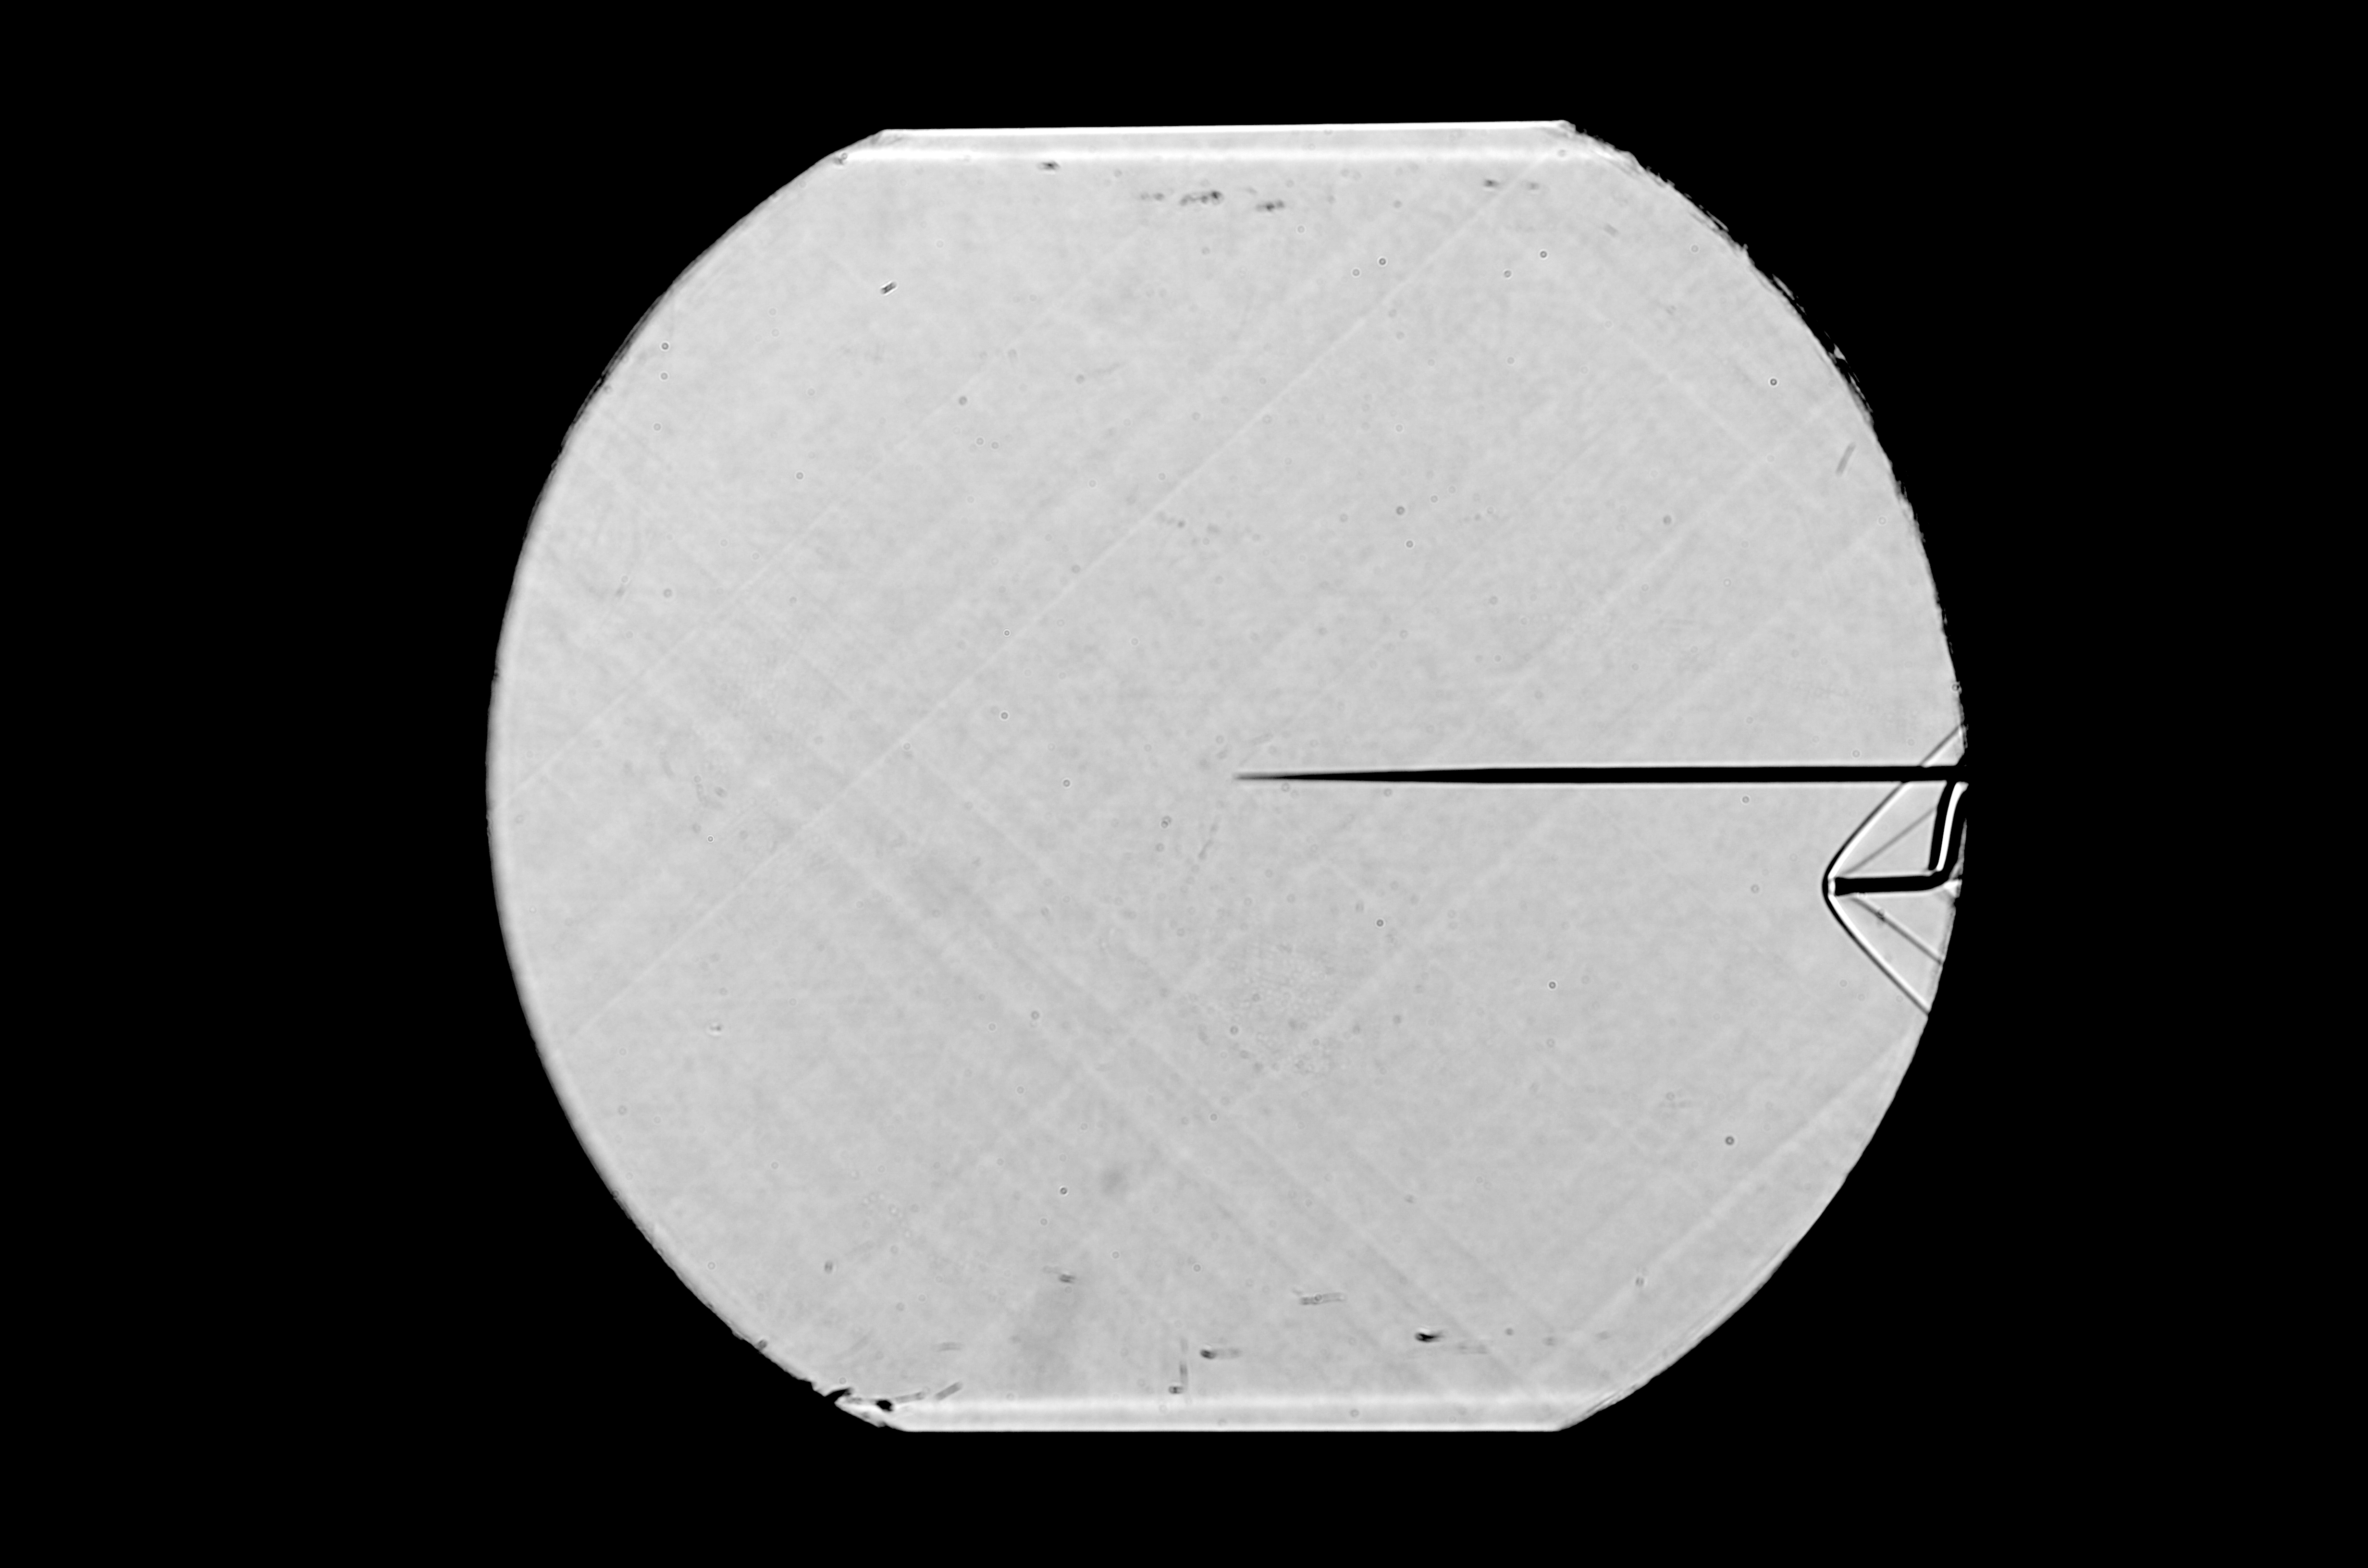
\includegraphics[width=0.8\textwidth]{working_state.jpg}
    \caption{Figure 2}
    \label{fig:figure7}
\end{figure}

\newpage

\begin{figure}[H]
    \centering
    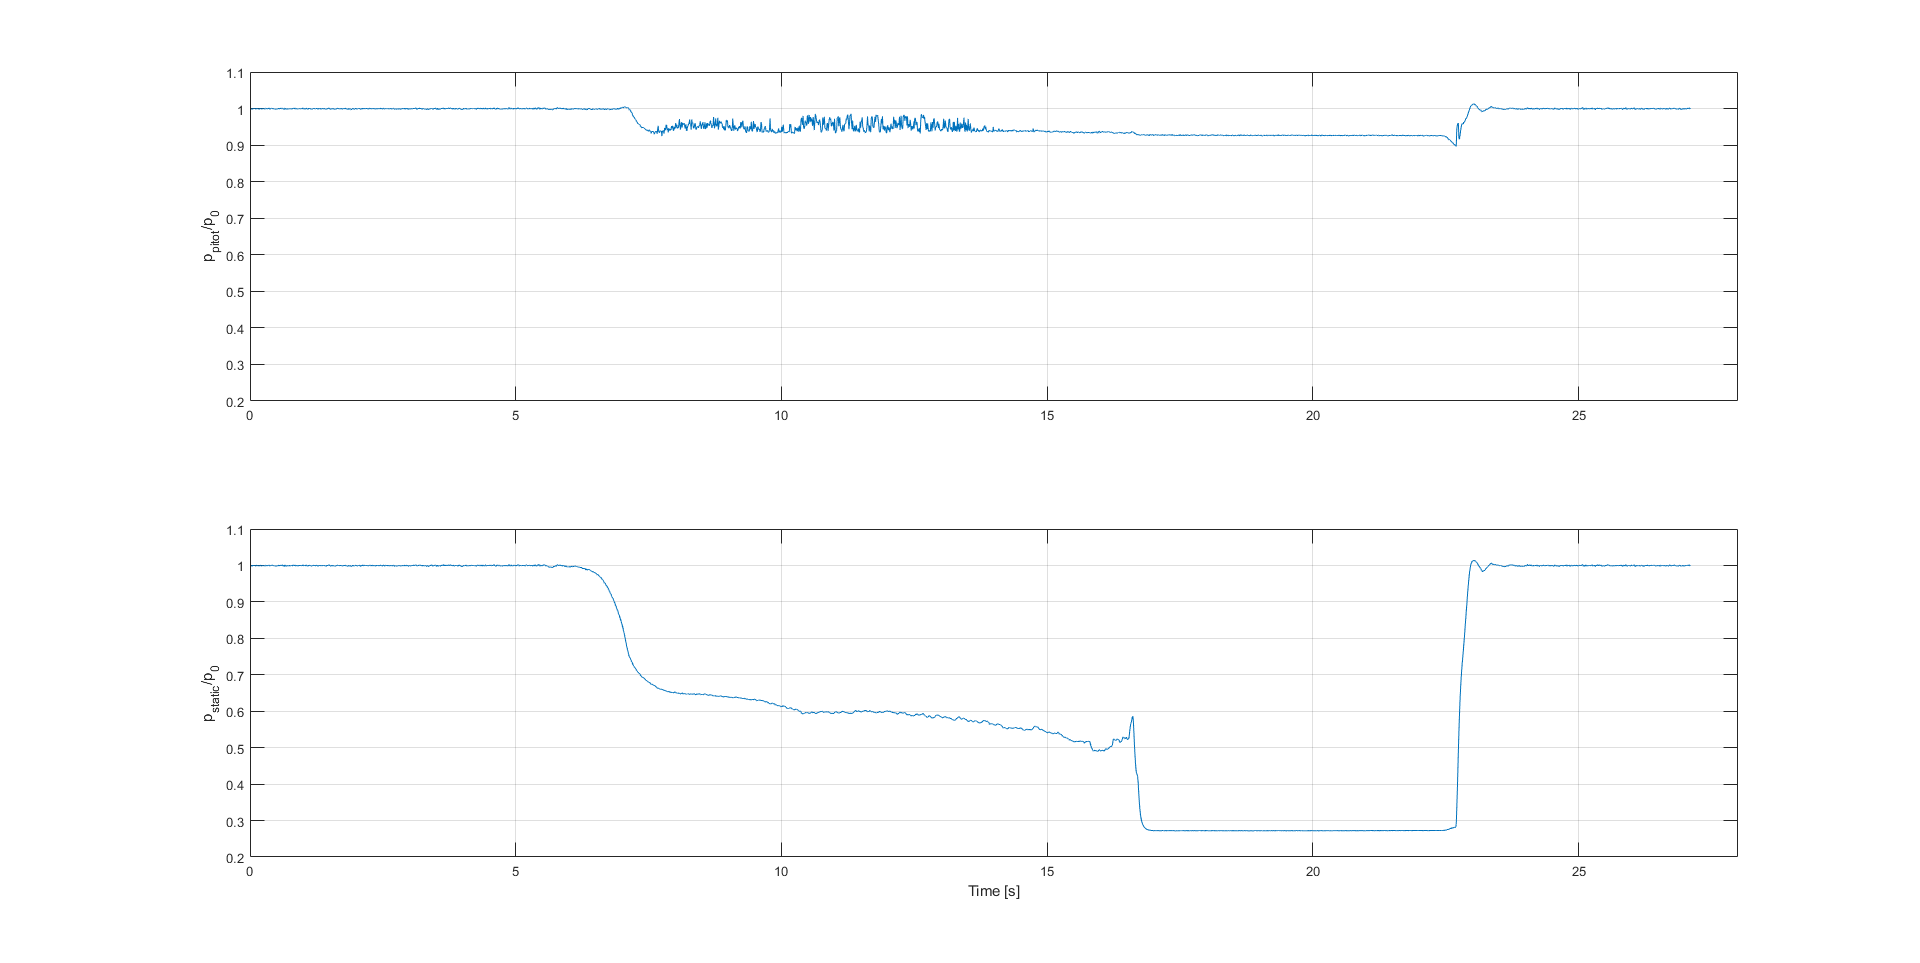
\includegraphics[width=0.8\textwidth]{tunnel_pressures.png}
    \caption{Figure 3}
    \label{fig:figure8}
\end{figure}

\newpage

\section{Discussion}

%interpret results and comment on anomalies

\subsection{Improvements}

\section{Conclusion}

From the experiments performed it can be observed that blah blah blah

\end{document}
